\documentclass[a4paper,12pt]{article}
%\usepackage[latin1]{inputenc}
\usepackage[spanish]{babel}
\usepackage{bm}
\usepackage{graphicx}
\usepackage{amsmath}
\setlength{\textheight}{235mm}
\setlength{\textwidth}{168mm}
\setlength{\oddsidemargin}{0pt}
\pagestyle{empty}
\spanishdecimal{.}
\begin{document}
\mbox{}\vspace*{-45mm}

{\centering
{\small\sc 
%Escuela Técnica Superior de Ingenieros de Caminos, Canales y Puertos (Madrid)\\*[4mm]
Máster Universitario en Ingeniería de Estructuras, Cimentaciones y Materiales}\\*[4mm]
{\Large\bf Método de los Elementos Finitos 24-25}\\*[4mm]
PRÁCTICA 3: Modelos de difusión \\*[4mm]
}

\vspace{3mm}

%%%%%
\noindent
La figura muestra la sección transversal de un río canalizado, en una zona en la que se ha construido un túnel provisional de $5$ m de longitud y sección cuadrada de $1$ m de lado. El extremo derecho del túnel está a la presión atmosférica. El terreno tiene un coeficiente de permeabilidad $k_1=k_2=2\cdot10^{-3}$ m/s y está confinado por pantallas impermeables y terreno igualmente impermeable.\\

Para analizar las filtraciones que se producen se realizará un modelo plano de elementos finitos que represente dicha sección transversal. La discretización a efectuar corresponde a elementos cuadrilateros lineales de cuatro
nodos de lado $0.25$ m.\\

Se pide:

\begin{itemize}
\item Analizar la distribución de presiones (altura piezométrica) y la distribución de velocidades horizontales y verticales.
\item Analizar la distribución de presiones (altura piezométrica) y la distribución de velocidades horizontales y verticales considerando $k_2=1\cdot 10^{-5}$.
\end{itemize}



\begin{center}
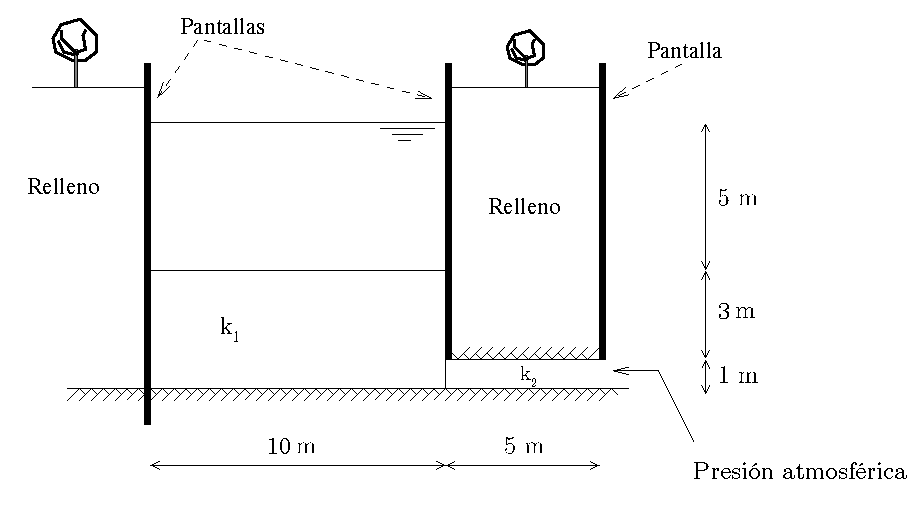
\includegraphics[width=0.85\textwidth]{practi2_b}
\end{center}


\vspace{3mm}

\hspace{20mm}\hrulefill$\star$\hrulefill\hspace{20mm}

\vspace{3mm}


Resultados del ejercicio con dos materiales:
\begin{itemize}
\item $h_A = 8.99$ m
\item $Pw_A = 78.4$ kPa
\item $q^x_A = 1.7\cdot 10^{-5}$ m/s (En el elemento marcado en el dibujo cercano a A.)
\item $Q_{out} = 1.7\cdot 10^{-5}$ m$^3$/s
\item $F^{p_w}_{AB} = 184.5$ kN

\end{itemize}

\end{document}
